\section{Appendix II}

\subsection{<<Fundamentals of Magnonics>>\cite{rezende2020fundamentals}}

    In <<Fundamentals of Magnonics>> the derivation of magnon dispersion is done in chapter~$3$~<<Quantum Theory of Spin Waves: Magnons>>.

    The Hamiltonian is defined on page~$72$, equation~\eqref{eq:fom-3.6} as follows:

    \begin{quote}
        \begin{equation}
            H = -g\mu_B\sum_iH_zS_i^z - J\sum_{i, \delta}\vec{S}_i \cdot \vec{S}_{i+\delta}, \label{eq:fom-3.6} \tag{3.6}
        \end{equation}
        where$\vec{S}_i$ is spin angular momentum operator as site $i$, <...> and $\vec{\delta}$ is the vector connecting site $i$ with its nearest neighbors. 
        <...> Notice also that the factor 2 in the exchange energy does not appear explicitly because each pair of spins is counted twice in the sum over lattice sites.
    \end{quote}

    The definition of the Hamiltonian (we ignore the Zeeman term) is the same as in~\eqref{eq:hh-main} with the following notation change:
    \begin{equation}
        \begin{matrix} 
            \vec{S}_{i+\delta} \rightarrow \vec{S}_j, & \sum_{i, \delta} \rightarrow \sum_{i,j}
        \end{matrix}
    \end{equation}
    therefore, no conversion is needed for parameters for this textbook.

    Magnon dispersion is provided on page $78$ in equations~\eqref{eq:fom-3.35}~and~\eqref{eq:fom-3.36}

    \begin{quote}
        \begin{equation}
            E_k = A_k = g\mu_B H_z + 2zJS(1 - \gamma_k), \label{eq:fom-3.35} \tag{3.35}
        \end{equation}
        where $\gamma_k$ is the structure factor given by
        \begin{equation}
            \gamma_k = \dfrac{1}{z}\sum_{\vec{\delta}}e^{\iu \vec{k}\cdot\vec{\delta}} \label{eq:fom-3.36} \tag{3.36}
        \end{equation}
    \end{quote}
    where $z$ is the number of neighbors ($n$ in the notation of this paper). $\gamma_k$ for the cubic system is (it is provided on page~$79$ in equation~\eqref{eq:fom-3.37}):
    \begin{quote}
        \begin{equation}
            \gamma_k = \dfrac{1}{3}(\cos(k_xa) + \cos(k_ya) + \cos(k_za)) \label{eq:fom-3.37} \tag{3.37}
        \end{equation}
    \end{quote}
    where $a$ is a lattice parameter ($l$ in the notation of this paper). The final equation from the \cite{rezende2020fundamentals} in the notation of this paper is
    \begin{equation}
        \hbar\omega(\mathbf{k}) = 2nJS\left(1 - \dfrac{1}{3}\left(\cos(k_xl) + \cos(k_yl) + \cos(k_zl)\right)\right)
        \label{eq:rezende}
    \end{equation}

    This equation is the same as equation~\eqref{eq:main-dispersion} ($n = 6$).

\subsection{<<Magnetism in condensed matter>>\cite{blundell2003magnetism}}
    The derivation of magnon dispersion for the ferromagnetic 1D chain is discussed in the section~$6.6.6$~<<Magnons>>.

    The definition of the Hamiltonian is provided on page~$122$ in equations~\eqref{eq:micm-6.9}~and~\eqref{eq:micm-6.10}
    \begin{quote}
        (1) We begin with a semiclassical derivation of the spin wave dispersion.
        First, recall the Hamiltonian for the Heisenberg model,
        \begin{equation}
            \hatH = -\sum_{\langle ij\rangle} J\hat{\mathbf{S}}_i \cdot \hat{\mathbf{S}}_j \label{eq:micm-6.9} \tag{6.9}
        \end{equation}
        (which is eqn. $6.4$) In a one-dimensional chain each spin has two neighbours, so the Hamiltonian reduces to
        \begin{equation}
            \hatH = -2J\sum_{i} \hat{\mathbf{S}}_i \cdot \hat{\mathbf{S}}_{i+1} \label{eq:micm-6.10} \tag{6.10}
        \end{equation}
    \end{quote}
    with the comment to the equation~($6.4$) on the page~$116$ being
    \begin{quote}
        where the constant $J$ is the exchange integral and the symbol $\langle ij \rangle$ below the $\sum$ denotes a sum over nearest neighbours. 
        The spins $\mathbf{S}_i$ are treated as three-dimensional vectors ...
    \end{quote}

    The definition of the Heisenberg model is found for the first time in the section~$4.2.1$ on the page~$76$ in equations~\eqref{eq:micm-4.7}~and~\eqref{eq:micm-4.8}:
    \begin{quote}
        This motivates the Hamiltonian of the Heisenberg model:
        \begin{equation}
            \hatH = -\sum_{ij}J_{ij}\mathbf{S}_i \cdot \mathbf{S}_j, \label{eq:micm-4.7} \tag{4.7}
        \end{equation}
        where $J_{ij}$ is the exchange constant between the $i^{\text{th}}$ and $j^{\text{th}}$ spins. 
        The factor of 2 is omitted because the summation includes each pair of spins twice. 
        Another way of writing eqn $4.7$ is 
        \begin{equation}
            \hatH = -2\sum_{i>j}J_{ij}\mathbf{S}_i \cdot \mathbf{S}_j, \label{eq:micm-4.8} \tag{4.8}
        \end{equation}
        where the $i > j$ avoids the <<double-counting>> and hence the factor of two returns. 
        Often it is possible to take $J_{ij}$ to be equal to a constant $J$ for nearest neighbours spins and to be $0$ otherwise.
    \end{quote}
    The equation~\eqref{eq:micm-6.9} corresponds to the definition in equation~\eqref{eq:micm-4.7} 
    and the equation~\eqref{eq:micm-6.10} corresponds to the definition in equation~\eqref{eq:micm-4.8}. 
    The definition in equation~\eqref{eq:micm-4.7} is the same as in equation~\eqref{eq:hh-main}, 
    therefore, no conversion of parameters is needed for this textbook.

    The Hamiltonian is solved specifically for the ferromagnetic 1D chain and not for the 3D cubic system with the final result (equation~\ref{eq:micm-6.20} on page~$123$ and equation~\ref{eq:micm-6.25} on page~$124$)
    \begin{quote}
        \begin{equation}
            \hbar\omega = 4JS(1 - \cos(qa)), \label{eq:micm-6.20} \tag{6.20}
        \end{equation}
        \begin{equation}
           E(q) = -2NS^2J + 4JS(1 - \cos(qa)), \label{eq:micm-6.25} \tag{6.25}
        \end{equation}
    \end{quote}
    which matches with the equations~\eqref{eq:zero-energy}~and~\eqref{eq:main-dispersion} if $n = 2$ is used and 1D-chain instead of 3D cubic system is considered. 
    Magnon dispersion from equation~\eqref{eq:micm-6.20} is plotted in the book on page~$123$ in figure~$6.12$ (Fig.~\ref{fig:micm-6.12}). 
    Path from $0$ to $\pi / a$ corresponds to the $\Gamma$-X path in Fig.~\ref{fig:main-dispersion}. If the parameters from this paper are substitute into the eq.~\eqref{eq:micm-6.20} then those two graphs are be exactly the same.
    \begin{quote}
        \begin{figure}[H]
            \centering
            \begin{subfigure}[b]{0.5\textwidth}
                \centering
                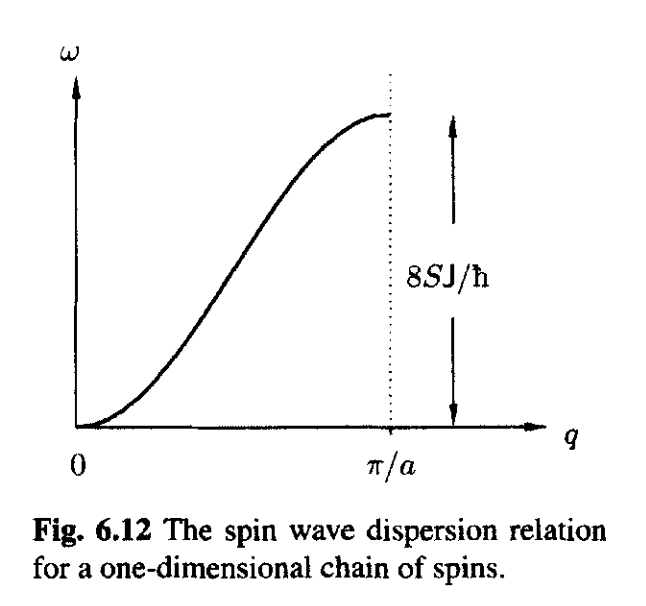
\includegraphics[height=6cm]{micm-6.12.png}
            \end{subfigure}
            \hfill
            \caption{Magnon dispersion plot from <<Magnetism in condensed matter>>.}
            \label{fig:micm-6.12}
        \end{figure}
    \end{quote}
    For the cubic system eq.~\ref{eq:micm-6.20} will look like:
    \begin{equation}
        \hbar\omega = 12JS(1 - \dfrac{1}{3}(\cos(q_xa) + \cos(q_ya) + \cos(q_za)))
    \end{equation}
    If it is to be rewritten with the notation of this paper it will look like ($n = 6$)
    \begin{equation}
        \hbar\omega = 2nJS(1 - \dfrac{1}{3}(\cos(k_xl) + \cos(k_yl) + \cos(k_zl)))
    \end{equation}

\subsection{<<Magnetisation oscillations and waves>>\cite{gurevich1996magnetization}}
    The derivation of magnon dispersion for the ferromagnet is discussed in the section~$7.4$~<<Elements of microscopic spin-wave theory>>.

    The definition of the Hamiltonian is provided on page~$205$ in equations~\eqref{eq:moaw-7.82}~and~\eqref{eq:moaw-7.82}

    \begin{quote}
        \begin{equation}
            \hatH = \gamma\hbar\sum_{f}\hat{S}_f^z - \sum_f\sum_{f^{\prime} \ne f} I_{ff^{\prime}}\mathbf{S}_f\mathbf{S}_{f^{\prime}} \label{eq:moaw-7.82} \tag{7.82}
        \end{equation}
        where $\mathbf{S}_f\mathbf{S}_{f^{\prime}} = \hat{S}_f^x\hat{S}_{f^{\prime}}^x + \hat{S}_f^y\hat{S}_{f^{\prime}}^y + \hat{S}_f^z\hat{S}_{f^{\prime}}^z$.
    \end{quote}
    The double counting is present in this Hamiltonian, thus, it is the same definition as in eq.~\eqref{eq:hh-main} of this paper with the following notation change:
    \begin{equation}
        \begin{matrix}
            f \rightarrow i, & 
            f^{\prime} \ne f \rightarrow j, & 
            I_{ff^{\prime}} \rightarrow J, & 
            \mathbf{S}_f \rightarrow \mathbf{S}_i, &
            \mathbf{S}_{f^{\prime}} \rightarrow \mathbf{S}_j
        \end{matrix}
    \end{equation}

    The dispersion law is provided in equation~\eqref{eq:moaw-7.99} on page~$209$
    \begin{quote}
        where $r_g = r_f - r_{f^{\prime}}$, $I_g \equiv I_{ff^{\prime}}$, and the last sum is over all lattice points except one, the initial. 
        The Hamiltonian ($7.98$) has the desired form of ($7.84$), and
        \begin{equation}
            \varepsilon_k(k) = \gamma\hbar H + 2S \sum_g [1 - exp(\iu \mathbf{k}\mathbf{r}_g)]I_g. \label{eq:moaw-7.99} \tag{7.99}
        \end{equation}
    \end{quote}

    For the cubic ferromagnet the textbook provides the figure~7.13 (Fig.~\ref{fig:moaw-7.13})
    \begin{quote}
        \begin{figure}[H]
            \centering
            \begin{subfigure}[b]{0.49\textwidth}
                \centering
                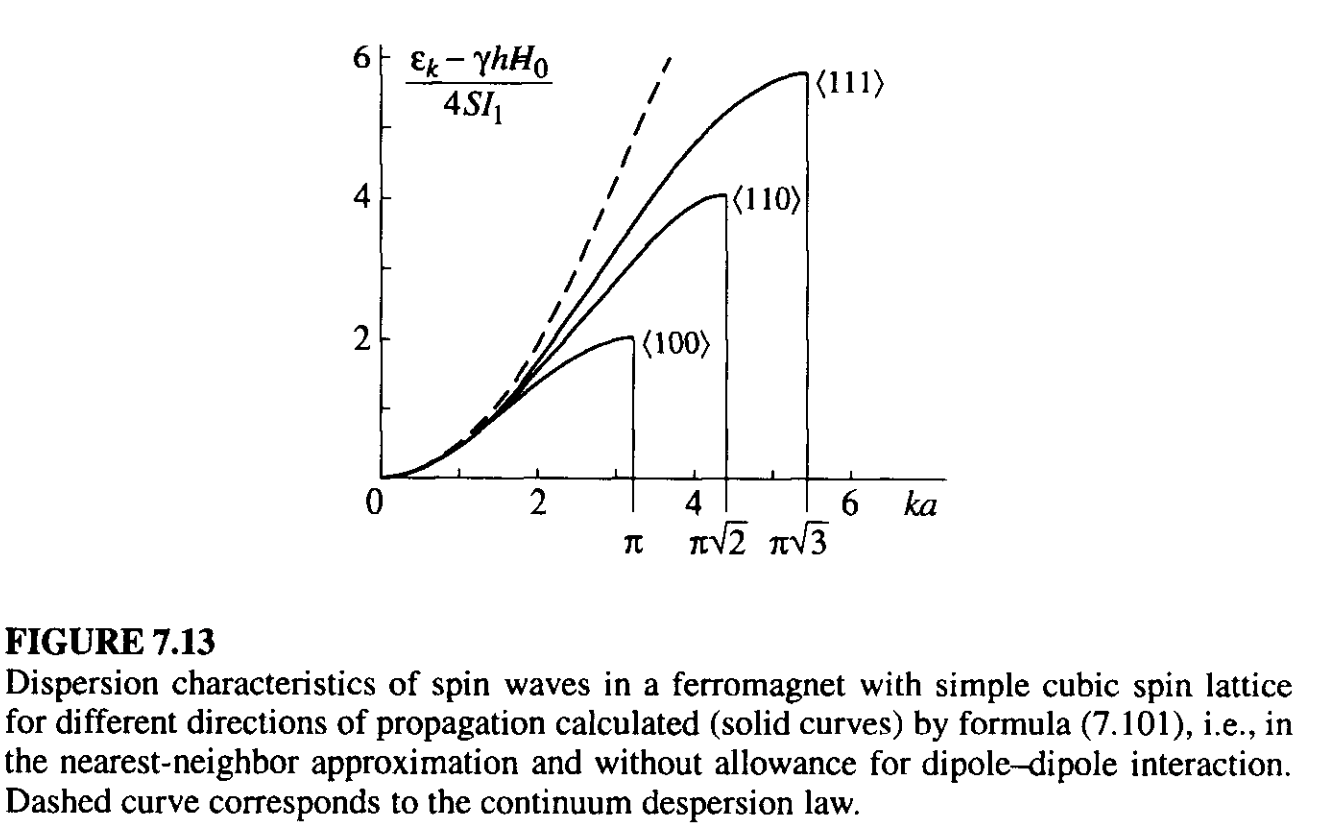
\includegraphics[height=6cm]{moaw-7.13.png}
                \caption{Original plot}
                \label{fig:moaw-7.13-original}
            \end{subfigure}
            \hfill
            \begin{subfigure}[b]{0.49\textwidth}
                \centering
                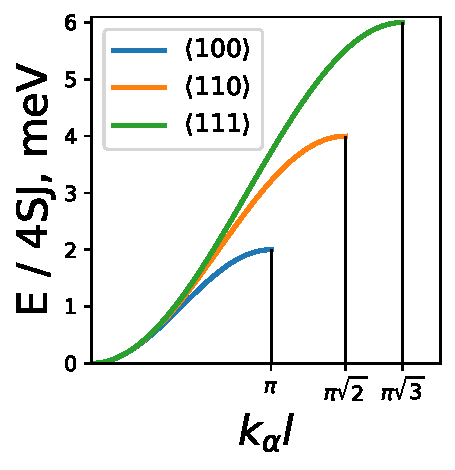
\includegraphics[height=6cm]{custom-moaw.pdf}
                \caption{Same plot with use of eq.~\eqref{eq:main-dispersion}}
                \label{fig:moaw-7.13-custom}
            \end{subfigure}
            \hfill
            \caption{Magnon dispersion plot from <<Magnetisation oscillations and waves>>.}
            \label{fig:moaw-7.13}
        \end{figure}
    \end{quote}
    In this picture curve~$\langle 100\rangle$ (from $0$ to $\pi$) corresponds to the path $\Gamma$-Y, 
    curve~$\langle 110\rangle$ (from $0$ to $\pi\sqrt{2}$) to the path $\Gamma$-M and
    curve~$\langle 111\rangle$ (from $0$ to $\pi\sqrt{3}$) to the path $\Gamma$-R 
    in the Fig.~\ref{fig:main-dispersion}. In Fig.~\ref{fig:moaw-7.13-custom} the same graph is plotted by using the equation for magnon dispersion from this paper.

    The dispersion law from eq.~\ref{eq:moaw-7.99} for the cubic system will be
    \begin{equation}
        \hbar\omega(\mathbf{k}) = 2SIn\left(1 - \dfrac{1}{3}\left(\cos(k_xr_x) + \cos(k_yr_y) + \cos(k_zr_z)\right)\right)
    \end{equation}
    where $g$ varies from $1$ to $6$ $r_g \in [r_x, -r_x, r_y, -r_y, r_z, -r_z]$ and $I_g = I$ for each $g$. 

    In the notation of this paper the dispersion law becomes ($n = 6$)
    \begin{equation}
        \hbar\omega(\mathbf{k}) = 2SJn\left(1 - \dfrac{1}{3}\left(\cos(k_xl) + \cos(k_yl) + \cos(k_zl)\right)\right)
    \end{equation}

\subsection{<<The Oxford Solid State Basics>>\cite{simon2013oxford}}
    The derivation of magnon dispersion for the ferromagnet is discussed in the exercise~$20.3$ for the Chapter~$20$~<<Spontaneous Magnetic Order: Ferro-, Antiferro-, and Ferri-Magnetism>>.

    The definition of the Hamiltonian is provided on page~$229$ in equations~\eqref{eq:ossb-20.6}~and~\eqref{eq:ossb-20.2}

    \begin{quote}
        Consider the Heisenberg Hamiltonian
        \begin{equation}
            \hatH = -\dfrac{1}{2}\sum_{\langle i,j \rangle} J \mathbf{S}_i \cdot \mathbf{S}_j + \sum_i g\mu_B \mathbf{B} \cdot \mathbf{S}_i \label{eq:ossb-20.6} \tag{20.6}
        \end{equation}
        and  for this exercise set $\mathbf{B} = 0$.
    \end{quote}

    For the first time Heisenberg Hamiltonian is defined on pages~$225-226$ in equation~\eqref{eq:ossb-20.2}
    \begin{quote}
        Note that we have included a factor of $1/2$ out front to avoid overcounting, since the sum actually counts both $J_{ij}$ and $J_{ji}$ (which are equal to each other).

        $\langle ... \rangle$

        One can use brackets $\langle i,j\rangle$ to indicate that $i$ and $j$ are neighbors:
        \begin{equation}
            \hatH = -\dfrac{1}{2}\sum_{\langle i,j \rangle} J_{ij} \mathbf{S}_i \cdot \mathbf{S}_j
        \end{equation}
        In a uniform system where each spin is coupled to its neighbors with the same strength, we can drop the indices from $J_{i,j}$ (since they all have the same value) and obtain the so-called \textit{Heisenberg Hamiltonian}
        \begin{equation}
            \hatH = -\dfrac{1}{2}\sum_{\langle i,j \rangle} J \mathbf{S}_i \cdot \mathbf{S}_j \label{eq:ossb-20.2} \tag{20.2}
        \end{equation}
        and  for this exercise set $\mathbf{B} = 0$.
    \end{quote}

    The double counting is present in this Hamiltonian, thus, it is the same definition as in eq.~\eqref{eq:hh-main} of this paper 
    with the additional factor of $1/2$, thus if we assume that definition of <<The Oxford Solid State Basics>> and this paper give the same Hamiltonian one have to 
    introduce the following substitution of exchange parameter in order to move to the definition of this paper:
    \begin{equation}
        J \rightarrow 2J \label{eq:ossb-sub}
    \end{equation}

    The dispersion law for the cubic system is provided  on page~$230$
    \begin{quote}
        $\triangleright$ Show that the dispersion curve for <<spin-waves>> of a ferromagnet is given by $\hbar\omega = \vert F(\mathbf{k})\vert$  where
        \begin{equation}
            F(\mathbf{k}) = g\mu_b\vert B \vert + JS\left(6 - 2\left(\cos(k_xa) + \cos(k_ya) + \cos(k_za)\right)\right)
        \end{equation}
        where we assume a cubic lattice
    \end{quote}

    In the notation of this paper (with the substitution~\eqref{eq:ossb-sub}) the dispersion law becomes ($n = 6$)
    \begin{equation}
        \hbar\omega(\mathbf{k}) = 2JSn\left(1 - \dfrac{1}{3}\left(\cos(k_xl) + \cos(k_yl) + \cos(k_zl)\right)\right)
    \end{equation}
\subsection{<<Magnetism and magnetic materials>>\cite{coey2010magnetism}}

\subsection{<<Rare earth magnetism>>\cite{jensen1991rare}}



